\documentclass[10pt, letterpaper]{report}
% !TeX program = xelatex
%==================PREAMBOLO=======================%
\usepackage[utf8]{inputenc}
\usepackage{psvectorian}
\usepackage{pgfplots}
\usepackage[Rejne]{fncychap}
\usepackage[export]{adjustbox}
\usepackage[T1]{fontenc}
\usepackage{lmodern}
\usepackage[shortlabels]{enumitem}
\usepackage{moresize}
\usepackage{graphicx} % Required for inserting images
\usepackage{hyperref}
\usepackage{listings}
\usepackage[table,xcdraw]{xcolor}
\usepackage{amssymb}
\usepackage{amsmath}
\usepackage[italian]{babel}
\usepackage{nicefrac, xfrac}
\usepackage{tikz}
\usepackage{mathrsfs} 
\usepackage{titletoc}
\usepackage{fancyhdr}
\usepackage{psvectorian,lipsum}
\usepackage{fourier-orns}
\usepackage{lipsum}
\usepackage[paper=a4paper,left=25mm,right=25mm,bottom=25mm,top=25mm]{geometry}
\definecolor{light-gray}{gray}{0.95}
\definecolor{cop}{HTML}{f7ecd7}
\definecolor{copAut}{HTML}{ababab}
\definecolor{copAut2}{HTML}{c3c3e6}
\definecolor{purcop}{HTML}{d0d3db}
\definecolor{sapienza}{HTML}{660f1d}
\definecolor{lightSapienza}{HTML}{e3d3d5}
\definecolor{darkgreen}{HTML}{008000}
\definecolor{cartaRiciclata}{HTML}{fcfcf7}
\newcommand{\redText}[1]{\color{red}#1\color{black}}
\newcommand{\code}[1]{\colorbox{light-gray}{\texttt{#1}}}
\newcommand{\codee}[1]{\colorbox{white}{\texttt{#1}}}
\newcommand{\K}{{\mathbb K}}
\newcommand{\notimplies}{%
  \mathrel{{\ooalign{\hidewidth$\not\phantom{=}$\hidewidth\cr$\implies$}}}}
\newcommand{\flowerLine}{ \begin{center}\decofourleft\hphantom{ }\decoone\hphantom{ }\decofourright\hphantom{}\hphantom{aa}
\decofourleft\hphantom{ }\decoone\hphantom{ }\decofourright\hphantom{}\hphantom{aa}
\decofourleft\hphantom{ }\decoone\hphantom{ }\decofourright\hphantom{}\hphantom{aa}
\decofourleft\hphantom{ }\decoone\hphantom{ }\decofourright\hphantom{}\hphantom{aa} 
\decofourleft\hphantom{ }\decoone\hphantom{ }\decofourright\hphantom{}\hphantom{aa}
\decofourleft\hphantom{ }\decoone\hphantom{ }\decofourright\hphantom{}\hphantom{aa}
\decofourleft\hphantom{ }\decoone\hphantom{ }\decofourright\hphantom{}\hphantom{aa}
\decofourleft\hphantom{ }\decoone\hphantom{ }\decofourright\hphantom{}\hphantom{aa}
\decofourleft\hphantom{ }\decoone\hphantom{ }\decofourright\hphantom{}\hphantom{aa}
\end{center}}
\definecolor{g}{RGB}{60, 50, 50}
\newcommand{\textg}[1]{\color{g}{\textbf{#1}}\color{black}}
\newcommand{\teo}[1]{{\large\color{sapienza}\textbf{Teorema #1 :\hphantom{a}}}}
\newcommand{\defi}[1]{{\large\color{sapienza}\textbf{Definizione #1 :\hphantom{a}}}}
\newcommand{\claim}[1]{{\color{sapienza}\textbf{Claim #1 :\hphantom{a}}}}
\newcommand{\lemma}[1]{{\color{sapienza}\textbf{Lemma #1 :\hphantom{a}}}}
\newcommand{\dimo}[1]{{\color{sapienza}\textbf{Dimostrazione #1 :\hphantom{a}}}}
\newcommand{\prop}[1]{{\color{sapienza}\textbf{Proposizione #1 :\hphantom{a}}}}
\newcommand\greybox[1]{%
  \vskip\baselineskip%
  \par\noindent\colorbox{light-gray}{%
    \begin{minipage}{\textwidth}#1\end{minipage}%
  }%
  \vskip\baselineskip%
}
\newcommand\sapbox[1]{%
  \vskip\baselineskip%
  \par\noindent\colorbox{lightSapienza}{%
    \begin{minipage}{\textwidth}#1\end{minipage}%
  }%
  \vskip\baselineskip%
}

\newcommand{\Z}{{\mathbb Z}}
\newcommand{\blank}{{\sqcup}}
\newcommand{\R}{{\mathbb R}}
\newcommand{\N}{{\mathbb N}}
\newcommand{\C}{{\mathbb C}}
\newcommand{\Sn}{{\mathcal S_n}}
\newcommand{\An}{{\mathcal A_n}}
\newcommand{\E}{{\mathcal E}}
\newcommand{\B}{{\mathcal B}}
\newcommand{\mcm}{{\text{mcm}}}
\newcommand{\rg}{{\text{rg}}}
\newcommand{\ve}{{\bar v}}
\newcommand{\spaz}{{\text{\hphantom{aa}}}}
\newcommand{\MCD}{{\text{MCD}}}
\newcommand{\tc}{{\text{ tale che }}}
\newcommand{\supp}{{\text{Supp}}}
\newcommand{\acc}{\\\hphantom{}\\}
\newcommand{\aut}{{\text{Aut}}}
\newcommand{\Span}{{\text{Span}}}
\newcommand{\End}{{\text{End}}}
\newcommand{\cen}{{\text{Centro}}}
\newcommand{\norm}{{\unlhd}}
\newcommand{\ciclS}{{\left \langle }}
\newcommand{\ciclE}{{\right \rangle }}
\newcommand{\boxedMath}[1]{\begin{tabular}{|c|}\hline \texttt{#1} \\ \hline\end{tabular} :}
\newcommand{\shell}[1]{\colorbox{black}{\textcolor{white}{\texttt{#1}}}}
\newcommand{\eqImportante}[1]{\begin{center}\huge\lefthand\hphantom{a}
    \normalsize\texttt{#1}
    \hphantom{aaa}\huge\righthand\end{center}}

\fancyhf{}
\pagestyle{fancy}
\usepackage{pgf-pie}  
\usetikzlibrary{positioning}

\renewcommand{\headrule}{%
\vspace{-8pt}\hrulefill
\raisebox{-2.1pt}{\quad\decothreeleft\decotwo\decothreeright\quad}\hrulefill}

%sta roba serve per il codice C
\definecolor{mGreen}{rgb}{0,0.6,0}
\definecolor{mGray}{rgb}{0.5,0.5,0.5}
\definecolor{mPurple}{rgb}{0.58,0,0.82}
\definecolor{backgroundColour}{rgb}{0.95,0.95,0.92}

\lstdefinestyle{CStyle}{
    backgroundcolor=\color{backgroundColour},   
    commentstyle=\color{mGreen},
    keywordstyle=\color{magenta},
    numberstyle=\tiny\color{mGray},
    stringstyle=\color{mPurple},
    basicstyle=\footnotesize,
    breakatwhitespace=false,         
    breaklines=true,                 
    captionpos=b,                    
    keepspaces=true,                 
    numbers=left,                    
    numbersep=5pt,                  
    showspaces=false,                
    showstringspaces=false,
    showtabs=false,                  
    tabsize=2,
    language=C
}
\lstdefinestyle{CppStyle}{
    backgroundcolor=\color{backgroundColour},   
    commentstyle=\color{mGreen}\ttfamily,
    morecomment=[l][\color{magenta}]{\#}
    keywordstyle=\color{blue}\ttfamily,
    numberstyle=\tiny\color{mGray},
    stringstyle=\color{red}\ttfamily,
    basicstyle=\ttfamily,
    breakatwhitespace=false,         
    breaklines=true,                 
    captionpos=b,                    
    keepspaces=true,                 
    numbers=left,                    
    numbersep=5pt,                  
    showspaces=false,                
    showstringspaces=false,
    showtabs=false,                  
    tabsize=2,
    language=C
}
\lstset{language=C++,
                basicstyle=\ttfamily,
                keywordstyle=\color{blue}\ttfamily,
                stringstyle=\color{red}\ttfamily,
                commentstyle=\color{green}\ttfamily,
                morecomment=[l][\color{magenta}]{\#}
}
%fine roba che serve per il codice C
\usepackage{minted}
 %TOGLI COMMENTO SE USI XELATEX
%\usepackage{fontspec}
\title{\jobname} %========TITOLO========%
\author{Marco Casu}
\date{\vspace{-5ex}}
\begin{document}

%==================COPERTINA=======================%
\begin{titlepage}
    \pagecolor{copAut}
\begin{center}
    %TOGLI COMMENTO SE USI XELATEX
   %\setmainfont{Palace Script MT}
   \HUGE Marco Casu\acc
    %\setmainfont{Grand Casino}
     %TOGLI COMMENTO SE USI XELATEX
    %\setmainfont{h Halfroad}
    \HUGE \decothreeleft\hphantom{ }{\fontsize{48}{50}\selectfont \jobname}\hphantom{ }\decothreeright
     %TOGLI COMMENTO SE USI XELATEX
   % \setmainfont{Times New Roman}
\end{center}
\thispagestyle{empty}
\begin{figure}[h]
    \centering{
        %l'immagine deve avere una risoluzione 2048x2048
        
\includegraphics[width=1\textwidth ]{images/Copertina.jpeg}
    }
\end{figure}
\vfill 
\centering 
\includegraphics[width=0.4\textwidth ]{../../../preamble/Stemma_sapienza.png} \acc
\centering \Large \color{sapienza}Facoltà di Ingegneria dell'Informazione,
Informatica e Statistica\\
Dipartimento di Informatica
\end{titlepage}

%===================FINE COPERTINA======================%
\newpage
\pagecolor{cartaRiciclata}%\setmainfont{Algerian}
\Large
Questo documento è distribuito sotto la licenza 
\color{blue}\href{https://www.gnu.org/licenses/fdl-1.3.txt}{GNU}\color{black},  
è un resoconto degli appunti (eventualmente integrati con libri di testo) tratti dalle lezioni del corso di \jobname
\hphantom{a}per la laurea 
triennale in Informatica. Se dovessi notare errori, ti prego di segnalarmeli.\acc 
Nota bene : Essendo questi appunti di un corso esterno alla facoltà di Informatica, 
è presente un capitolo "Complementi" che può risultare utile al lettore.
\newpage %\setmainfont{Times New Roman}
\normalsize
\tableofcontents 
\newpage

%==================FOOTER e HEADER=======================%
\fancyhf{}
\fancyhead[L]{\nouppercase{\leftmark}}
\fancyhead[R]{Sezione \thesection}
\fancyfoot[C]{\thepage}
\fancyfoot[L]{Appunti di \jobname}
\fancyfoot[R]{ Marco Casu}
%\fancyfoot[R]{\setmainfont{Palace Script MT}\huge Marco Casu \setmainfont{Times New Roman}}
%==================FOOTER e HEADER=======================%

%Ricorda del comando \flowerLine per separare le sottosezioni. Le sezioni si separano nelle diverse pagine

%==================INIZIO======================%
\chapter{Complementi}
\section{La Trasformata di Laplace} 
La trasformata di Laplace è una \textit{trasformata integrale}, nello specifico, è una 
funzione che associa ad una funzione di variabile reale, una funzione di variabile 
complessa.\acc 
\defi{(Trasformata di Laplace)} : Sia $f$ una funzione di variabile reale, nulla 
in $(-\infty,0)$, si chiama trasformata di Laplace di $f$ la funzione 
$$ \mathcal{L}[f](p)=\int_0^{+\infty} e^{-px}f(x)\ dx \ \ \ \ p\in \C$$
Essendo $p = \alpha + i\beta$ una variabile complessa, la funzione integranda si può riscrivere 
$$\int_0^{+\infty} e^{-px}f(x)\ dx = 
\int_0^{+\infty} e^{-(\alpha + i\beta)x}f(x)\ dx$$
Ricordando l'identità di Eulero $$ e^{ix}=\cos(x)+i\sin(x)$$
Si ha 
\begin{eqnarray}
    e^{-(\alpha + \beta i)x} = e^{-\alpha x}\cdot e^{-\beta i x} =\\ 
    e^{-\alpha x}\cdot \Big(
    \cos(-\beta x)+ i \sin(-\beta x)    
    \Big) = e^{-\alpha x}\cdot \Big(
        \cos(\beta x)- i \sin(\beta x)    
        \Big) = \\ 
        e^{-\alpha x}\cos(\beta x)- i e^{-\alpha x}\sin(\beta x)
\end{eqnarray}
Quindi $$ \mathcal{L}[f](p)=\mathcal{L}[f](\alpha + i\beta)=
\int_0^{+\infty} e^{-(\alpha + i\beta)x}f(x)\ dx=
$$
$$
\int_0^{+\infty} e^{-\alpha x}\cos(\beta x)f(x)-ie^{-\alpha x}\sin(\beta x)f(x)\ dx =$$
$$ 
\int_0^{+\infty} e^{-\alpha x}\cos(\beta x)f(x)\ dx-i\int_0^{+\infty}e^{-\alpha x}\sin(\beta x)f(x)\ dx
$$
Se l'integrale $\mathcal{L}[f](\alpha + i\beta)$ converge per un certo
 $\alpha \in \R$, allora converge per $p = \alpha + i\beta$ per ogni altro $\beta \in \R$. Se per 
 $f$ esiste almeno un $p\in\C$ tale che $\mathcal{L}[f](p)<\infty$, allora $f$ si dice 
 \textit{trasformabile secondo Laplace}.\acc
 In generale, se $\mathcal{L}[f](p)<\infty$ per $p=p_0$, allora è definita anche nel semipiano 
 complesso $$\{p\in \C \ |\ \Re(p)>\Re(p_0)\}$$
 Sia $\alpha_0$ l'estremo inferiore dell'insieme $\{\alpha \in \R \ |\ \mathcal{L}[f](p)<\infty\land \Re(p)>\alpha\}$, allora 
 il semipiano $\{p\in \C \|\ \Re(p)>\alpha_0\}$ è detto \textbf{semipiano di convergenza}.
 \begin{center}
    \includegraphics[width=0.6\textwidth ]{images/semiPianoConv.eps}
 \end{center}
 Vediamo un esempio di trasformata, si consideri $$ 
 H(x)=\begin{cases}
    1 \text{ se }x\ge 0\\ 0 \text{ altrimenti }
 \end{cases}
 $$
 \begin{center}
 \begin{figure}[h!]
    \centering
    \begin{tikzpicture}[scale=0.7, transform shape]
        \begin{axis}[
        ymin=-3,
        ymax = 3,
        xmin=-3,
        xmax = 3,
        axis lines = center,
        xtick distance=1, ytick distance=1,
        grid style=dashed,
        ymajorgrids=true,
        xmajorgrids=true,
        xlabel = \(\),
        ylabel = {\(\)},
        ]
        %Below the red parabola is defined
        \addplot [
        domain=0:3,
        samples=20,
        color=blue,
        ]
        {1};
        \end{axis}
        \end{tikzpicture}
        \caption{Funzione di Heaviside}
\end{figure}
\end{center}
Si calcola 
$$ \mathcal{L}[H](p)=\int_0^{+\infty}e^{-px}\cdot 1 \ dx = 
\lim_{T\rightarrow+\infty}\mathcal{L}[H](p)=\int_0^{T}e^{-px}\cdot 1 \ dx = 
\lim_{T\rightarrow+\infty}\begin{bmatrix}
    -\dfrac{e^{-px}}{p}
\end{bmatrix}_0^T=$$
$$\lim_{T\rightarrow+\infty} -\dfrac{e^{-pT}}{p} - \Big[-\dfrac{e^{-p0}}{p}\Big] =  
\lim_{T\rightarrow+\infty} -\dfrac{e^{-pT}}{p} +\dfrac{1}{p}=\frac{1}{p}$$
Il cui semipiano di convergenza risulta essere $\Re(p)>0$.
\subsection{Proprietà della Trasformata}
\subsubsection{Linearità}
La trasformazione di Laplace gode della proprietà di \textit{linearità}, siano $f(p)$ e $g(p)$ due funzioni 
trasformabili, siano $\lambda,\mu \in \C$ due costanti complesse, se la funzione 
$\lambda \cdot f(p)+\mu \cdot g(p)$ è trasformabile, allora 
$$ 
\mathcal{L}[\lambda \cdot f+\mu \cdot g](p)=\lambda\mathcal{L}[f](p)+\mu\mathcal{L}[g](p)
$$
Il semipiano di convergenza sarà uguale all'intersezione dei due semipiani di convergenza delle funzioni 
di partenza, più precisamente se \begin{itemize}
    \item $f$ ha come semipiano di convergenza $\Re(p)>\alpha$
    \item $g$ ha come semipiano di convergenza $\Re(p)>\beta$
    \item allora $\lambda \cdot f+\mu \cdot g$ ha come semipiano di convergenza $\Re(p)>\max\{\beta,\alpha\}$
\end{itemize}
\subsubsection{Ritardo}
Sia $f$ una funzione trasformabile, si consideri una costante reale $a>0$, la funzione $g(x)=f(x-a)$ è detta 
funzione \textit{ritardata}.\begin{center}
\begin{figure}[h!]\centering
    \includegraphics[width=0.6\textwidth ]{images/funRit.eps}
    \caption{funzione ritardata}
 \end{figure}\end{center}
Per il calcolo della trasformata di $g(x)=f(x-a)$ si considera il cambio di variabile $$\begin{matrix}
    t=x-a\\ x=t+a
\end{matrix} $$
Si ricordi come, se $f$ è nulla in $(-\infty,0)$, allora $g$ sarà nulla in $(0,a)$.
$$ 
\mathcal{L}[g](p)=\int_0^{+\infty}e^{-px}g(x)\ dx =\int_a^{+\infty}e^{-px}f(x-a)\ dx  =
\int_a^{+\infty}e^{-p(t+a)}f(t)\ dx = 
$$ 
$$ 
\int_a^{+\infty}e^{-pt-pa}f(t)\ dx 
= \int_a^{+\infty}e^{-pt}e^{-pa}f(t)\ dx = e^{-pa}\int_a^{+\infty}e^{-pt}f(t)\ dx = 
e^{-pa}\mathcal{L}[f](p)$$
Dunque si ricavano le cosiddette \textit{formule del ritardo} : 
$$ 
\mathcal{L}[f(x-a)](p)=e^{-pa}\mathcal{L}[f(x)](p)
$$ $$ 
\mathcal{L}[e^{ax}f(x)](p)=\mathcal{L}[f](p-a)
$$
\subsubsection{Trasformazione di una derivata e di una primitiva}
La seguente proprietà risulta cruciale nell'utilizzo della trasformata di Laplace per la risoluzione di 
equazioni differenziali. Le dimostrazioni dei seguenti risultati non saranno trattate in quanto non 
sono argomento di questo corso.\acc 
Sia $f$ una funzione derivabile, la cui derivata è continua in $[0,\infty)$. Sia inoltre $f'$ trasformabile, con 
semipiano di convergenza $\Re(p)>\alpha$, allora anche $f$ è trasformabile, ha semipiano di 
convergenza $\Re(p)>\max\{\alpha,0\}$, e vale la seguente identità :
\eqImportante{$
\mathcal{L}[f'](p)=p\mathcal{L}[f](p)-f(0)
$}
Si generalizza per derivate di ordine maggiore 
$$ 
\mathcal{L}[f''](p)=p^2\mathcal{L}[f](p)-pf(0)-f'(0)
$$
Analogamente, sia $F(x)=\int_0^x f(t)\ dt$, se $f$ è trasformabile ed ha semipiano di convergenza  $\Re(p)>\alpha$, 
allora anche $F$ lo è, ha semipiano di convergenza $\Re(p)>\max\{\alpha,0\}$ e vale che 
\eqImportante{$
\mathcal{L}[F](p)=\dfrac{1}{p}\mathcal{L}[f](p)
$}
\subsubsection{Convoluzione}
Siano $f$ e $g$ due funzioni integrabili secondo Riemann e nulle in $(-\infty,0)$, l'operatore $*$ detto \textbf{convoluzione} è 
definito nel modo seguente 
$$ (f*g)(x)=\int_0^{+\infty}f(x-t)g(t)\ dt=\int_0^{+\infty}f(t)g(x-t)\ dt$$
Se $f$ è trasformabile, e $|g|$ lo è, nello stesso semipiano, allora $f*g$ è trasformabile e vale 
$$ \mathcal{L}[f*g](p)=\mathcal{L}[f](p)\cdot\mathcal{L}[g](p)$$
\subsubsection{Derivata ed Integrale della trasformata di Laplace}
Essendo $\mathcal{L}[f](p)=\int_0^{+\infty}f(x)e^{-px}\ dx$
si ha 
 $$\frac{d}{dp}\mathcal{L}[f](p)=\frac{d}{dp}\int_0^{+\infty}f(x)e^{-px}\ dx$$
  $$\frac{d}{dp}\mathcal{L}[f](p)=\int_0^{+\infty}\frac{d}{dp}(f(x)e^{-px})\ dx$$
   $$\frac{d}{dp}\mathcal{L}[f](p)=\int_0^{+\infty}-xf(x)e^{-px}\ dx$$
    $$\frac{d}{dp}\mathcal{L}[f](p)=\mathcal{L}[-xf(x)](p)$$
    Generalizzando, per ogni $n\ge 0$ 
    \eqImportante{$\displaystyle\frac{d^n}{dp^n}\mathcal{L}[f](p)=\mathcal{L}[-(1)^nx^nf(x)](p)$}
\textbf{Esempio di calcolo} : Si vuole trovare  
$$ \mathcal{L}[x\sin(\omega x)](p)$$
Essendo 
$$  \mathcal{L}[\sin(\omega x)](p) = \frac{\omega}{p^2+\omega^2}$$
Ho che 
$$\mathcal{L}[x\sin(\omega x)](p) = - \frac{d}{dp}\mathcal{L}[\sin(\omega x)](p) = 
- \frac{d}{dp}\Big(\frac{\omega}{p^2+\omega^2}\Big)=\frac{2p\omega}{(p^2+\omega^2)^2}$$
Trascurando il procedimento, la formula per l'integrale di una trasformata è la seguente 
\eqImportante{$\displaystyle
\int_p^{+\infty}\mathcal{L}[f](s)\ ds = \mathcal{L}[\frac{f(x)}{x}](p)
$}
\subsection{Trasformata inversa}
La funzione che associa ad ogni funzione trasformabile la sua trasformata, è iniettiva, se $F(p)$ è una 
trasformata di Laplace, esiste un unica funzione $f$ tale che $\mathcal{L}[f](p)=F(p)$. Data $F$, è possibile 
ottenere la funzione di base su cui si è effettuata la trasformata, tale operazione è detta 
\textit{trasformazione inversa} di Laplace, si indica con $\mathcal{L}^{-1}$
$$ \mathcal{L}[f]=F$$
$$ \mathcal{L}^{-1}[F]=f$$
Le formule di trasformazione derivate dalle proprietà (raggruppate alla fine di questa sezione), se lette 
al contrario valgono come formule di anti-trasformata.\acc 
\textbf{Esempio di calcolo} : Ricordando che $\mathcal{L}[e^{-ax}](p)=\frac{1}{p+a}$, si vuole calcolare 
la trasformata inversa di 
$$\frac{2}{p+3} $$
\begin{eqnarray}
  \mathcal{L}^{-1}[\frac{2}{p+3}](x)=  \\ 
  2\cdot \mathcal{L}^{-1}[\frac{1}{p+3}](x) = \\ 
  2\cdot e^{-3x}\cdot H(x)
\end{eqnarray}
Una funzione risultante da un anti trasformata va moltiplicata per la funzione di Heaviside $H(x)$ in 
quanto deve essere nulla in $(-\infty,0)$.
\textbf{Esempio di calcolo} : Si vuole trovare l'anti trasformata di 
$$ F(p)=\dfrac{1}{p(p^2+1)}$$
Riscrivo la funzione 
$$ 
\dfrac{1}{p(p^2+1)}=\dfrac{1}{p^3+p}=\dfrac{1}{p}-\dfrac{p}{p^2+1}
$$
Applicando la linearità ho 
\begin{eqnarray}\mathcal{L}^{-1}[\dfrac{1}{p}-\dfrac{p}{p^2+1}](x)= 
\mathcal{L}^{-1}[\dfrac{1}{p}](x)-\mathcal{L}^{-1}[\dfrac{p}{p^2+1}](x)=\\ 
H(x)-\cos(x)\cdot H(x) = H(x)(1-\cos(x))
\end{eqnarray}
\subsection{Trasformate note}
\begin{center}
    \begin{tabular}{ccc}
        \rowcolor[HTML]{C0C0C0} 
        Funzione & Trasformata & Semipiano di convergenza \\ 
        \rowcolor[HTML]{EFEFEF} 
        $1$        & $\dfrac{1}{p}$          & $\Re(p)>0$        \\ 
        \rowcolor[HTML]{EFEFEF} 
                &            &         \\ 
        \rowcolor[HTML]{EFEFEF} 
        $e^{-ax}$        & $\dfrac{1}{p+a}$            & $\Re(p)>-\Re(a)$         \\  
        \rowcolor[HTML]{EFEFEF} 
                &            &         \\ 
        \rowcolor[HTML]{EFEFEF} 
        $x$        & $\dfrac{1}{p^2}$           & $\Re(p)>0$           \\  
        \rowcolor[HTML]{EFEFEF} 
                &            &         \\ 
        \rowcolor[HTML]{EFEFEF} 
        $x^n$        &  $\dfrac{n!}{p^{n+1}}$         & $\Re(p)>0$  $n\in\N$       \\  
        \rowcolor[HTML]{EFEFEF} 
                &            &         \\ 
        \rowcolor[HTML]{EFEFEF} 
        $\sin(\omega x)$        & $\dfrac{\omega}{p^2+\omega^2}$           & $\Re(p)>0$            \\  
        \rowcolor[HTML]{EFEFEF} 
                &            &         \\ 
        \rowcolor[HTML]{EFEFEF} 
        $\cos(\omega x)$         & $\dfrac{p}{p^2+\omega^2}$                & $\Re(p)>0$            \\  
        \rowcolor[HTML]{EFEFEF} 
                &            &         \\ 
        \rowcolor[HTML]{EFEFEF} 
        $\delta$        & $1$           & $p\in\C$        \\   
        \rowcolor[HTML]{EFEFEF} 
                &            &         \\ 
        \rowcolor[HTML]{EFEFEF} 
       $\cosh(ax)$        & $\dfrac{p}{p^2-a^2}$           & $\Re(p)>|\Re(a)|$          \\  
       \rowcolor[HTML]{EFEFEF} 
               &            &         \\ 
        \rowcolor[HTML]{EFEFEF} 
        $\sinh(ax)$       &  $\dfrac{a}{p^2-a^2}$             & $\Re(p)>|\Re(a)|$         \\ 
        \end{tabular}
\end{center}
\subsubsection{Funzione di trasferimento}
Come già accennato, la trasformata di Laplace è utile nella risoluzione di equazioni differenziali. Si consideri 
il seguente problema di Cauchy
$$ a_0y''(t)+a_1y'(t)+a_2y(t)=b(t)\ \ \ \ \begin{cases}
    y(0)=\alpha\\ y'(0)=\beta
\end{cases}$$ 
Si applica la trasformata all'equazione, ottenendo 
$$ \mathcal{L}[a_0y''+a_1y'+a_2y](p)=\mathcal{L}[b](p)$$
si applica la linearità 
$$a_0\mathcal{L}[y''](p)+a_1\mathcal{L}[y'](p)+a_2\mathcal{L}[y](p)=\mathcal{L}[b](p)$$
Chiamo $$ \mathcal{L}[y](p) = Y(p)\ \ \ \ \ \ \mathcal{L}[b](p)=B(p)$$
ed applico le proprietà della trasformazione di una derivata 
$$a_0(p^2Y(p)-p\alpha-\beta)+a_1(pY(p)-\alpha)+a_2Y(p)=B(p) $$
$$a_0p^2Y(p)-a_0p\alpha-a_0\beta+a_1pY(p)-a_1\alpha+a_2Y(p)=B(p) $$
esplicito $Y(p)$ : 
$$ Y(p)(a_0p^2+a_1p+a_2)=B(p)+a_0p\alpha+a_0\beta+a_1\alpha $$
$$ Y(p)=\frac{1}{(a_0p^2+a_1p+a_2)}B(p)+a_0p\alpha+a_0\beta+a_1\alpha $$
Pongo 
$$S(p)=\frac{1}{(a_0p^2+a_1p+a_2)} $$
Tale $S$ è detta \textbf{funzione di trasferimento}, se le condizioni iniziali sono entrambe nulle, ossia 
$\alpha=\beta=0$, si ha 
$$ Y(p)=S(p)\cdot B(p)$$
$$ \mathcal{L}[y](p)=S(p)\cdot \mathcal{L}[b](p) $$
Ricordando la convoluzione di una trasformata, si ha che 
$$y(t)=\mathcal{L}^{-1}[S\cdot B](t)$$ 
$$y(t)=\mathcal{L}^{-1}[S](t)*\mathcal{L}^{-1}[B](t)$$ 
$$y(t)=\mathcal{L}^{-1}[S](t)*b(t)$$ 
Le seguenti formule hanno un significato fisico notevole, supponiamo che vi sia un sistema fisico 
caratterizzato da un ingresso $b(t)$, ed un uscita $y(t)$, ad esempio, $b(t)$ è una forza, e 
$y(t)$ il moto di una particella. Trovare esplicitamente il moto $y$ non è banale, è possibile quindi 
applciare la trasformata, passando nel dominio complesso di Laplace, per poi risolvere l'equazione ed 
applicare l'anti trasformata, trovando così il moto.\begin{center}
    \begin{figure}[h!]\centering
        \includegraphics[width=0.5\textwidth ]{images/funTrasf.eps}
        \caption{Funzione di Trasferimento}
     \end{figure}\end{center}
La funzione $S(p)$ quindi caratterizza totalmente il sistema fisico nel dominio di Laplace, in quanto basta 
moltiplicarla alla trasformata del segnale in ingresso per ottenere la trasformata del segnale in 
uscita.\acc 
\textbf{Esempio di calcolo} : Si consideri il seguente problema di Cauchy
$$ y''(t)+2y'(t)+y(t)=e^{-2t}\ \ \ \ \begin{cases}
    y(0)=1\\ y'(0)=0
\end{cases}$$ 
Si applica la trasformata di Laplace, ottenendo 
$$ Y(p)(p^2+2p+1)=\frac{1}{p+2}+p+2$$
$$ Y(p)=\frac{1}{(p^2+2p+1)}\Big(\frac{1}{p+2}+p+2\Big)$$
ho che 
$$ y(t)=\mathcal{L}^{-1}[\frac{1}{(p^2+2p+1)}\Big(\frac{1}{p+2}+p+2\Big)](t)$$
Trovo l'anti trasformata : 
$$ \mathcal{L}^{-1}[\frac{1}{(p^2+2p+1)}](t)*\mathcal{L}^{-1}[\Big(\frac{1}{p+2}+p+2\Big)](t)$$
calcolo separatamente i due termini
$$ 
\mathcal{L}^{-1}[\Big(\frac{1}{p+2}+p+2\Big)](t)=
H(t)e^{-2t}+\mathcal{L}^{-1}[p](t)+2\mathcal{L}^{-1}[1](t) = 
$$
$$ 
H(t)e^{-2t}+2\delta(t)
$$
passo al secondo termine 
$$
\mathcal{L}^{-1}[\frac{1}{(p^2+2p+1)}](t)=\mathcal{L}^{-1}[\frac{1}{(p+1)(p+1)}](t)
=H(t)te^{-t}$$
si ha 
$$y(t)=H(t)te^{-t}*H(t)e^{-2t}+2\delta(t)$$
\color{red}ho sbalgiato qualcosa, procedimento da rivedere\color{black}
\end{document}